\documentclass[12pt,a4paper]{report}
\usepackage[utf8]{inputenc}

%\documentclass{article}
\usepackage{graphicx}
\graphicspath{ {./P10_P11_atteliUNtabulas/} }

\usepackage{geometry}
 \geometry{
 a4paper,
 total={170mm,257mm},
 left=20mm,
 top=20mm,
 }

\begin{document}
\begin{titlepage}
	\centering
	\large{Rīgas tehniskā universitāte\\Elektronikas un telekomunikāciju fakultāte\\Elektronikas pamatu katedra\\}
	\vspace{4.5cm}
	{\scshape\Large LaTex apgūšana (P10\_P11 uzdevums)\par}
	\vspace{0.5cm}
	{\huge\bfseries Sprieguma dalītājs\\\par}
	\vspace{11cm}

	\begin{flushright}
	    {\Large Vladimirs Fedorovičs\\REBM02, 041RDB182\par}
	\end{flushright}

	\vfill
	{2020. gada jūlijs}
\end{titlepage}

\begin{center}
{\huge\bfseries Darba mērķi\par}
\end{center}
\vspace{0.5cm}
\setlength{\parindent}{0cm}
• Aprakstīt sprieguma dalītāja shēmas izveidi ar gEDA rīkiem P09 uzdevumam.\\
• Iemācīties veidot vienkāršus LaTeX dokumentus.\\
• Iemācīties ievietot formulas, attēlus un tabulas.
\vspace{2cm}


\begin{center}
{\huge\bfseries Dotie parametri\par}
\end{center}
\begin{center}
\begin{table}[!ht]
\begin{tabular}{| c || c |}
\hline
 \textbf{Elements} & \textbf{Vērtība} \\ [0.5ex] 
 \hline\hline
\hline
$R_{1}, \Omega$ & 9,0 \\ \hline
$R_{2}, \Omega$ & 3,0 \\ \hline
$V_1, V$ & 18,2 \\ \hline
\end{tabular}
\end{table}
\end{center}

{\large\bfseries Shēmas zīmēšana \emph{gschem}\par}
\begin{itemize}
  \item Lai atvērtu programmu ierakstīsim Linux terminālā komandu \emph{gschem}.
  \item Tālāk zīmēsim tāpat ka LTSpice, skatīties zemāk:\\
        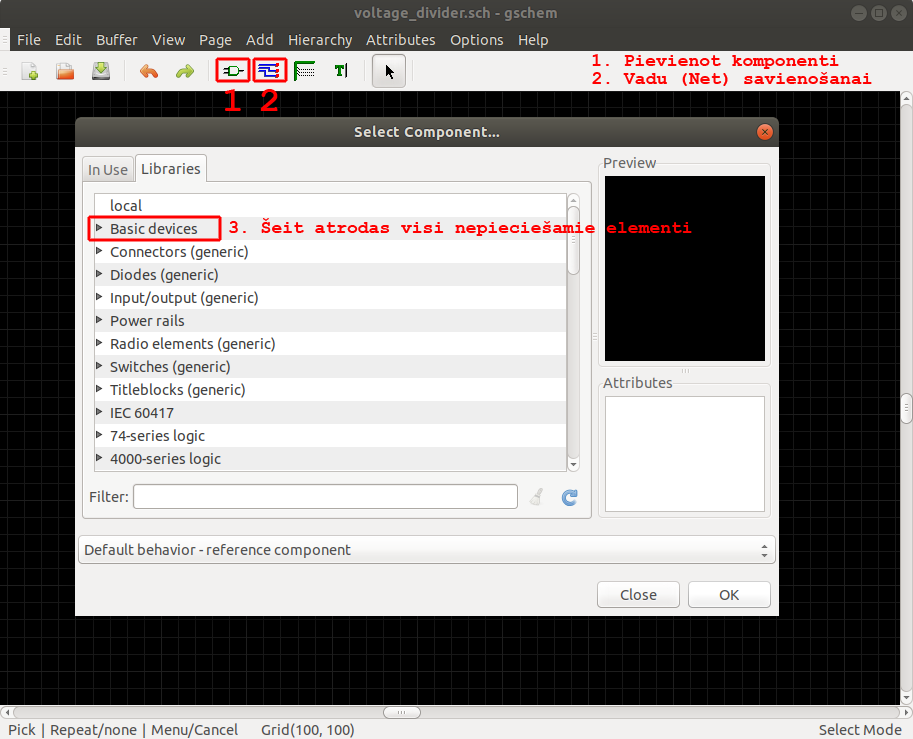
\includegraphics[scale=0.4]{1}\\
        Ar 1. ikonu pievienosim nepieciešamos elementus un ar 2. ikonu – savienosim elementus savās starpā.
  \item Vērtību un nosaukumu piešķiršana vizualizēta zemāk:\\
        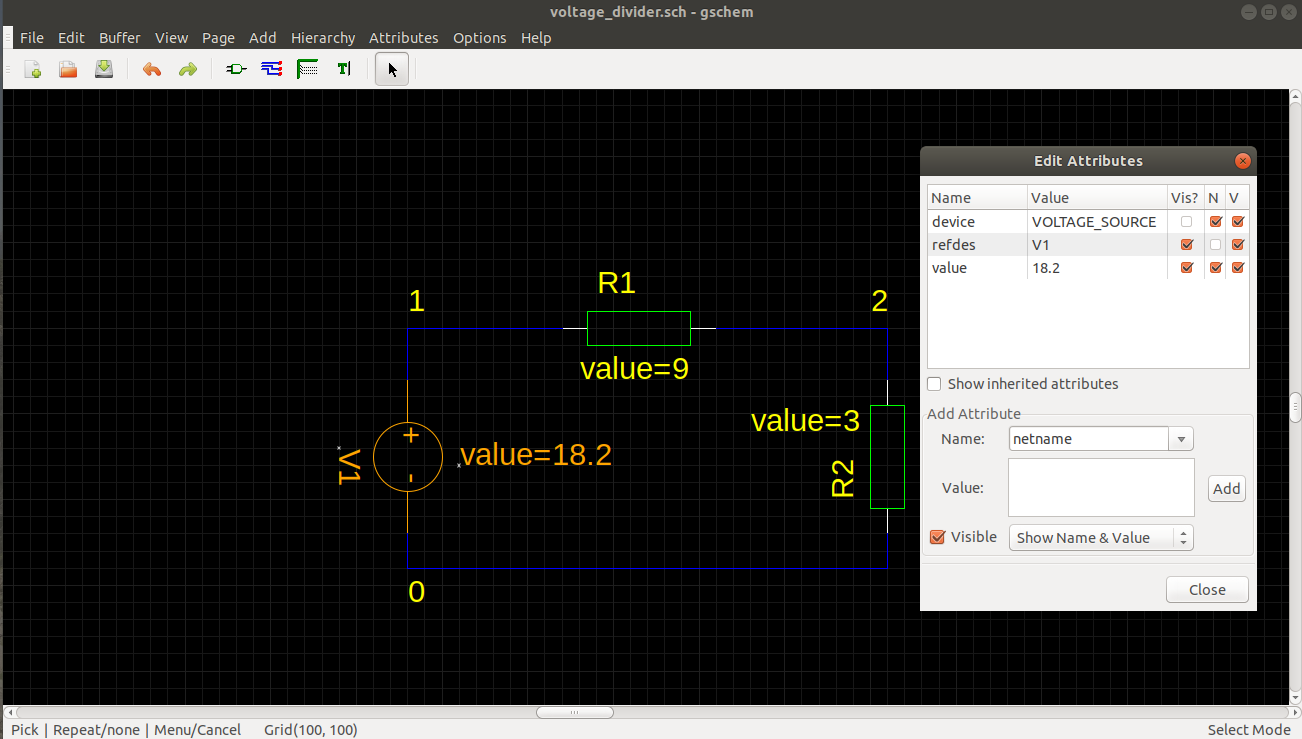
\includegraphics[scale=0.3]{2}\\
        Klikšķinot uz elementa ar labo peles taustiņu atvēras parametru lodziņš, kur jau pievienojam paremetrus izvēloties atbilstošos \emph{Add Attribute} zonā un pievienojot ar pogu \emph{Add}: \emph{refdes} – emelenta nosaukums, \emph{value} – vērtība.
  \item Tad pievienojam ZEMES punktu, klikšķinot ar labo peles taustiņu uz vēlamā mezgla un izvēloties no saraksta [\emph{Add attribute...}], \emph{value} ierakstam "0":\\
        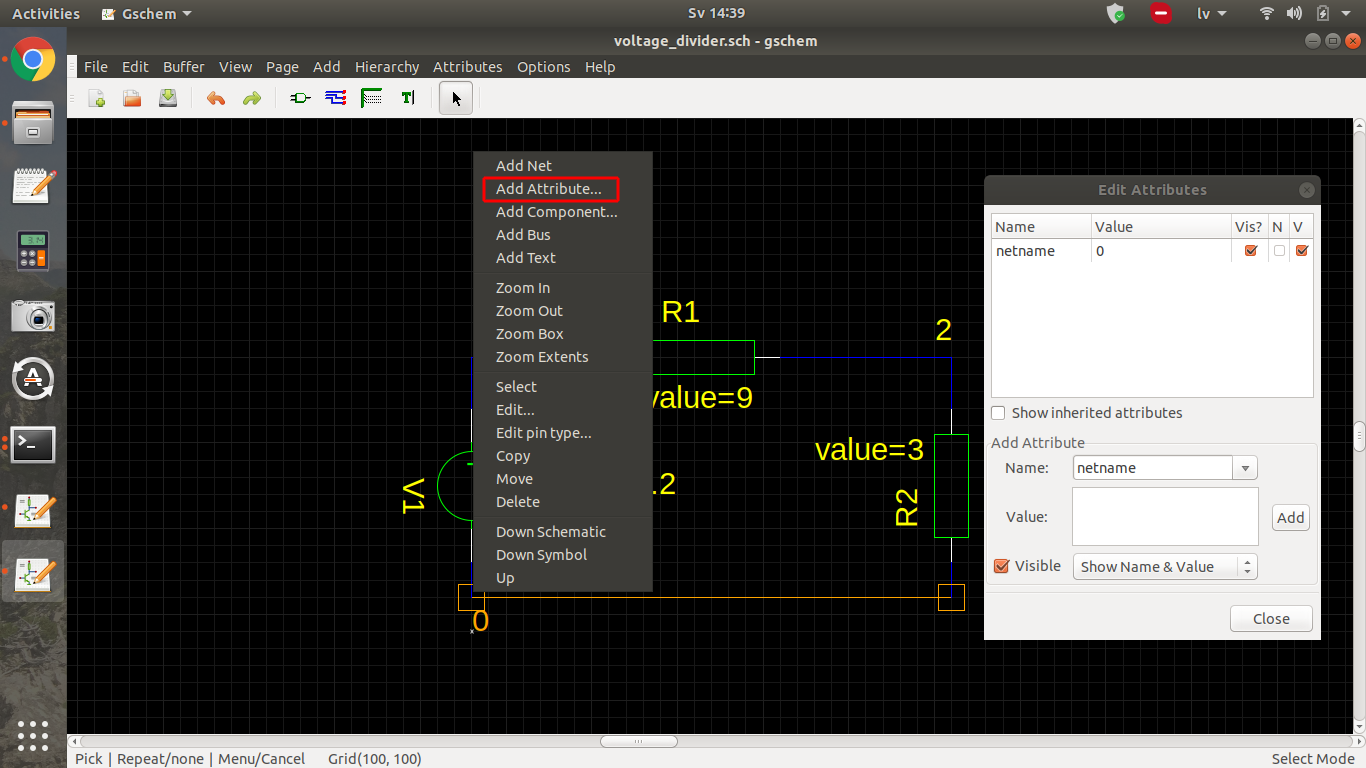
\includegraphics[scale=0.3]{3}\\
        Tādā veidā pievienojam arī pārējos mezglus piešķirot tiem nosaukumus, piem., "1" un "2".\\
  \item Saglabāsim failu ar nosaukumu \emph{voltage\_divider.sch}\\
        \pagebreak
  \item Lai saglabātu shēmu kā attēlu, spiežam \emph{File} un [\emph{Write Image...}] un izvēlamies nepieciešamo formātu (PNG, EPS, utt.):\\
         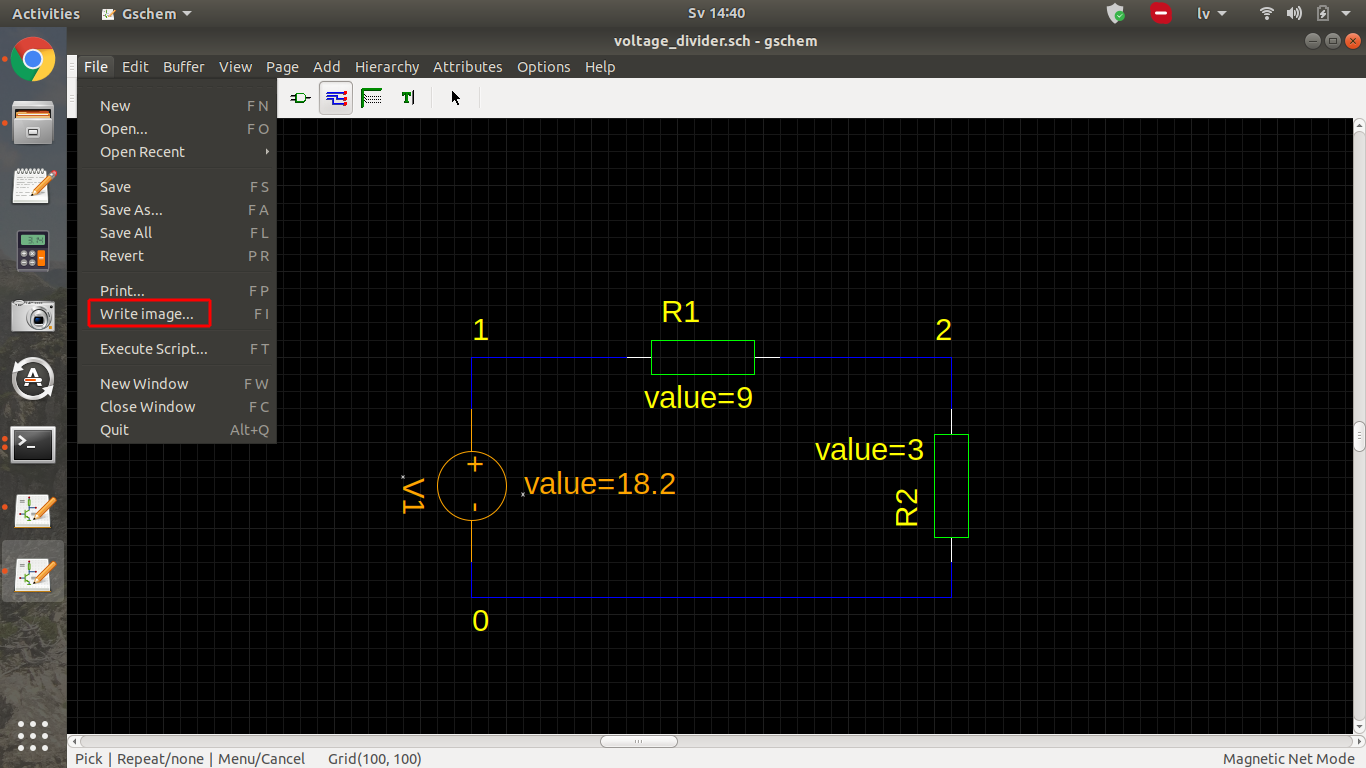
\includegraphics[scale=0.3]{4}\\
  \item Šādi izskatās noeksportēts attēls:\\
         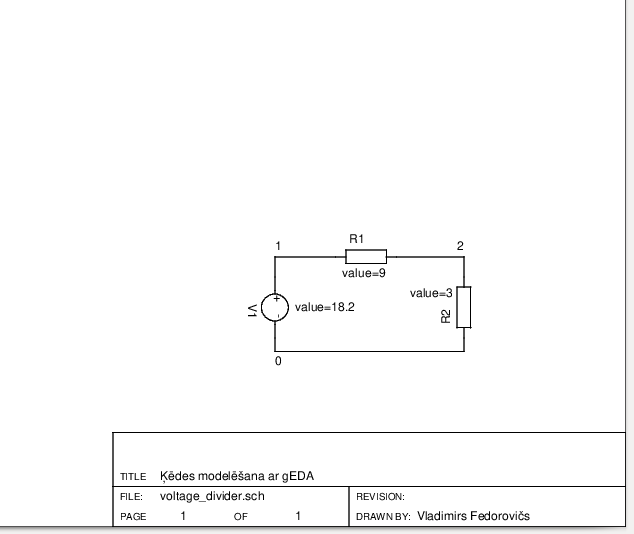
\includegraphics[scale=0.3]{P10_P11_atteliUNtabulas/voltage_divider.png}
  \item Iziesiem no programmas aizvērot to ar krustiņu (vai kā savādāk).\\       
\end{itemize}

{\large\bfseries Shēmas simulēšana \emph{ngspice}\par}
\begin{itemize}
    \item Lai varētu nodarboties ar simālāciju, sākumā izveidosim failu ar paplašinājumu *.net. Terminālā ierakstīsim komandu [\emph{gnetlist}] ar paramatiem [\emph{-g spice -0 GalaFailaNosaukums.net IzejasFailaNosaukums.sch}]. Mūsu gadījumā \emph{IzejasFailaNosaukums.sch} būs \emph{voltage\_divider.sch}.\\
    \item Palaižam programmu ar komandridiņu \emph{ngspice}.\\
    \item Tālāk ielādējam mūsu *.net failu iekšā ar komandu: \emph{source GalaFailaNosaukums.net}.\\
    \item Tad tāpat kā LTSpice izmantojam \emph{tran} direktīvu. Šeit tā būs komandrindiņa: \emph{tran 0.01ms 10ms}\\
    \item Tad uzzīmējam pirmā un otrā mezgla spriegumus izmantojot komandas \emph{plot "1"} un \emph{plot "2"} un saglabājam tos nospiežot atbilstošo podziņu \emph{hardcopy}:\\
          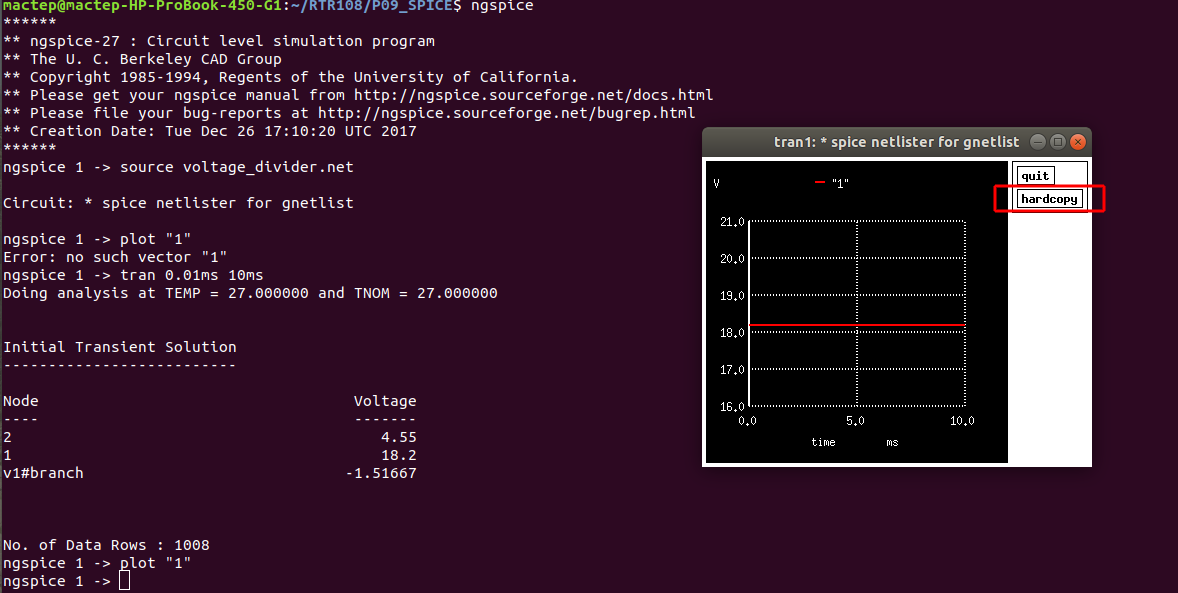
\includegraphics[scale=0.3]{5}\\
    \item Lai saglabāt krāsainu attēlu, tad pirms \emph{plot} komandas nepieciešams ievadīt komandu \emph{set hcopypscolor = 0}.\\
    \item Šādi izskatās abu mezglu spriegumu grafiki:\\
          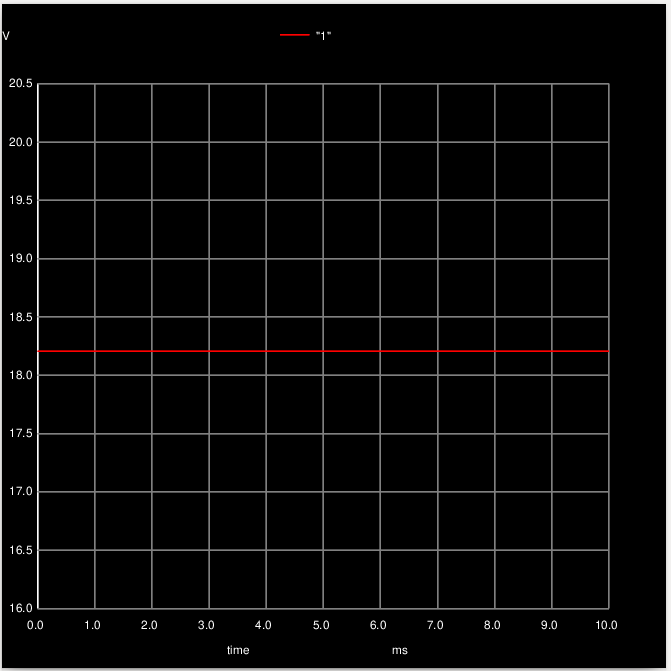
\includegraphics[scale=0.35]{P10_P11_atteliUNtabulas/voltage_divider_Vnode1.png} 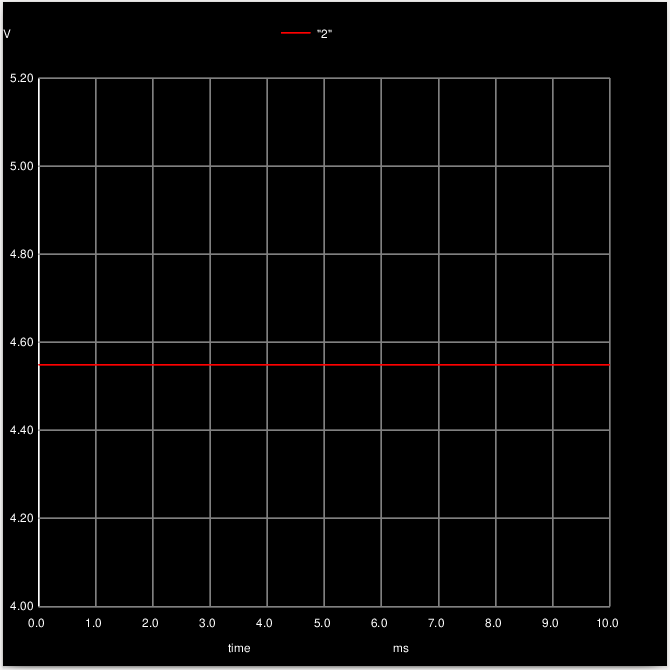
\includegraphics[scale=0.35]{P10_P11_atteliUNtabulas/voltage_divider_Vnode2.png}
\end{itemize}
\end{document}
